%% V1.0
%% by Gabriel Garcia, gabrcg@gmail.com
%% This is a template for Udacity projects using IEEEtran.cls

%% Be Udacious!


\documentclass[10pt,journal,compsoc]{IEEEtran}

\usepackage[pdftex]{graphicx}    
\usepackage{cite}
\usepackage{multirow}
\usepackage{adjustbox}
\hyphenation{op-tical net-works semi-conduc-tor}


\begin{document}

\title{Robotic Inference}



\author{Reinaldo Ossuna}

\markboth{Inference project, Robotics Nanodegree Program, Udacity}%
{}
\IEEEtitleabstractindextext{%

\begin{abstract}
  In this project we use the NVIDIA Deep Learning GPU Training System (DIGITS) to retrain several pretained models to classify two
  different datasets.
\end{abstract}

% Note that keywords are not normally used for peerreview papers.
\begin{IEEEkeywords}
Robot, Udacity, DIGITS, NVIDIA, DeepLearning.
\end{IEEEkeywords}}


\maketitle
\IEEEdisplaynontitleabstractindextext
\IEEEpeerreviewmaketitle
\section{Introduction}
\label{sec:introduction}

\IEEEPARstart{T}{raffic} signs classisification is a challeging problem and there is already many solution proposed in the
academicy field\cite{Stallkamp2012}\cite{Lim2017}\cite{Ciresan2012}\cite{Escalera1997}. The Germany Traffic Recognition Benchmark (GTSRB)\cite{Houben-IJCNN-2013} is a large dataset with multi-category classification
provided to the academics to study more this field.
  The goal in this project is to use the already known models, like AlexNet or GoogLeNet to classify tree traffic signs.





\section{Background}

In the first inference using the supplied dataset,the GoogLenet\cite{Iino2014} and the AlexNet\cite{YannLeCun1998} was tested with
differents optimizers and learning rate decay. In this fase we saw a big difference in both models and how the
optimizers and learning decays can interfere in final Inference.


\section{Data Acquisition}
The dataset was collected using a cellphone camera (Samsung S8 Picture Size 18.5:9, 4032$\times$1960 7.9M) multiple background
was used to better aurgementation of the images. In average we had 60 images per categorie, this value was not enough for
training, for better performace of the model we used some libraries in the python to make some augmentation in the
dataset and resize the images to 256$\times$256. In the end we had almost 4500 images per categorie.

\begin{figure}[thpb]
      \centering
      \includegraphics[width=\linewidth]{exdata.jpg}
      \caption{Example of the dataset}
      \label{fig:dataset1}
\end{figure}

\begin{figure}[thpb]
      \centering
      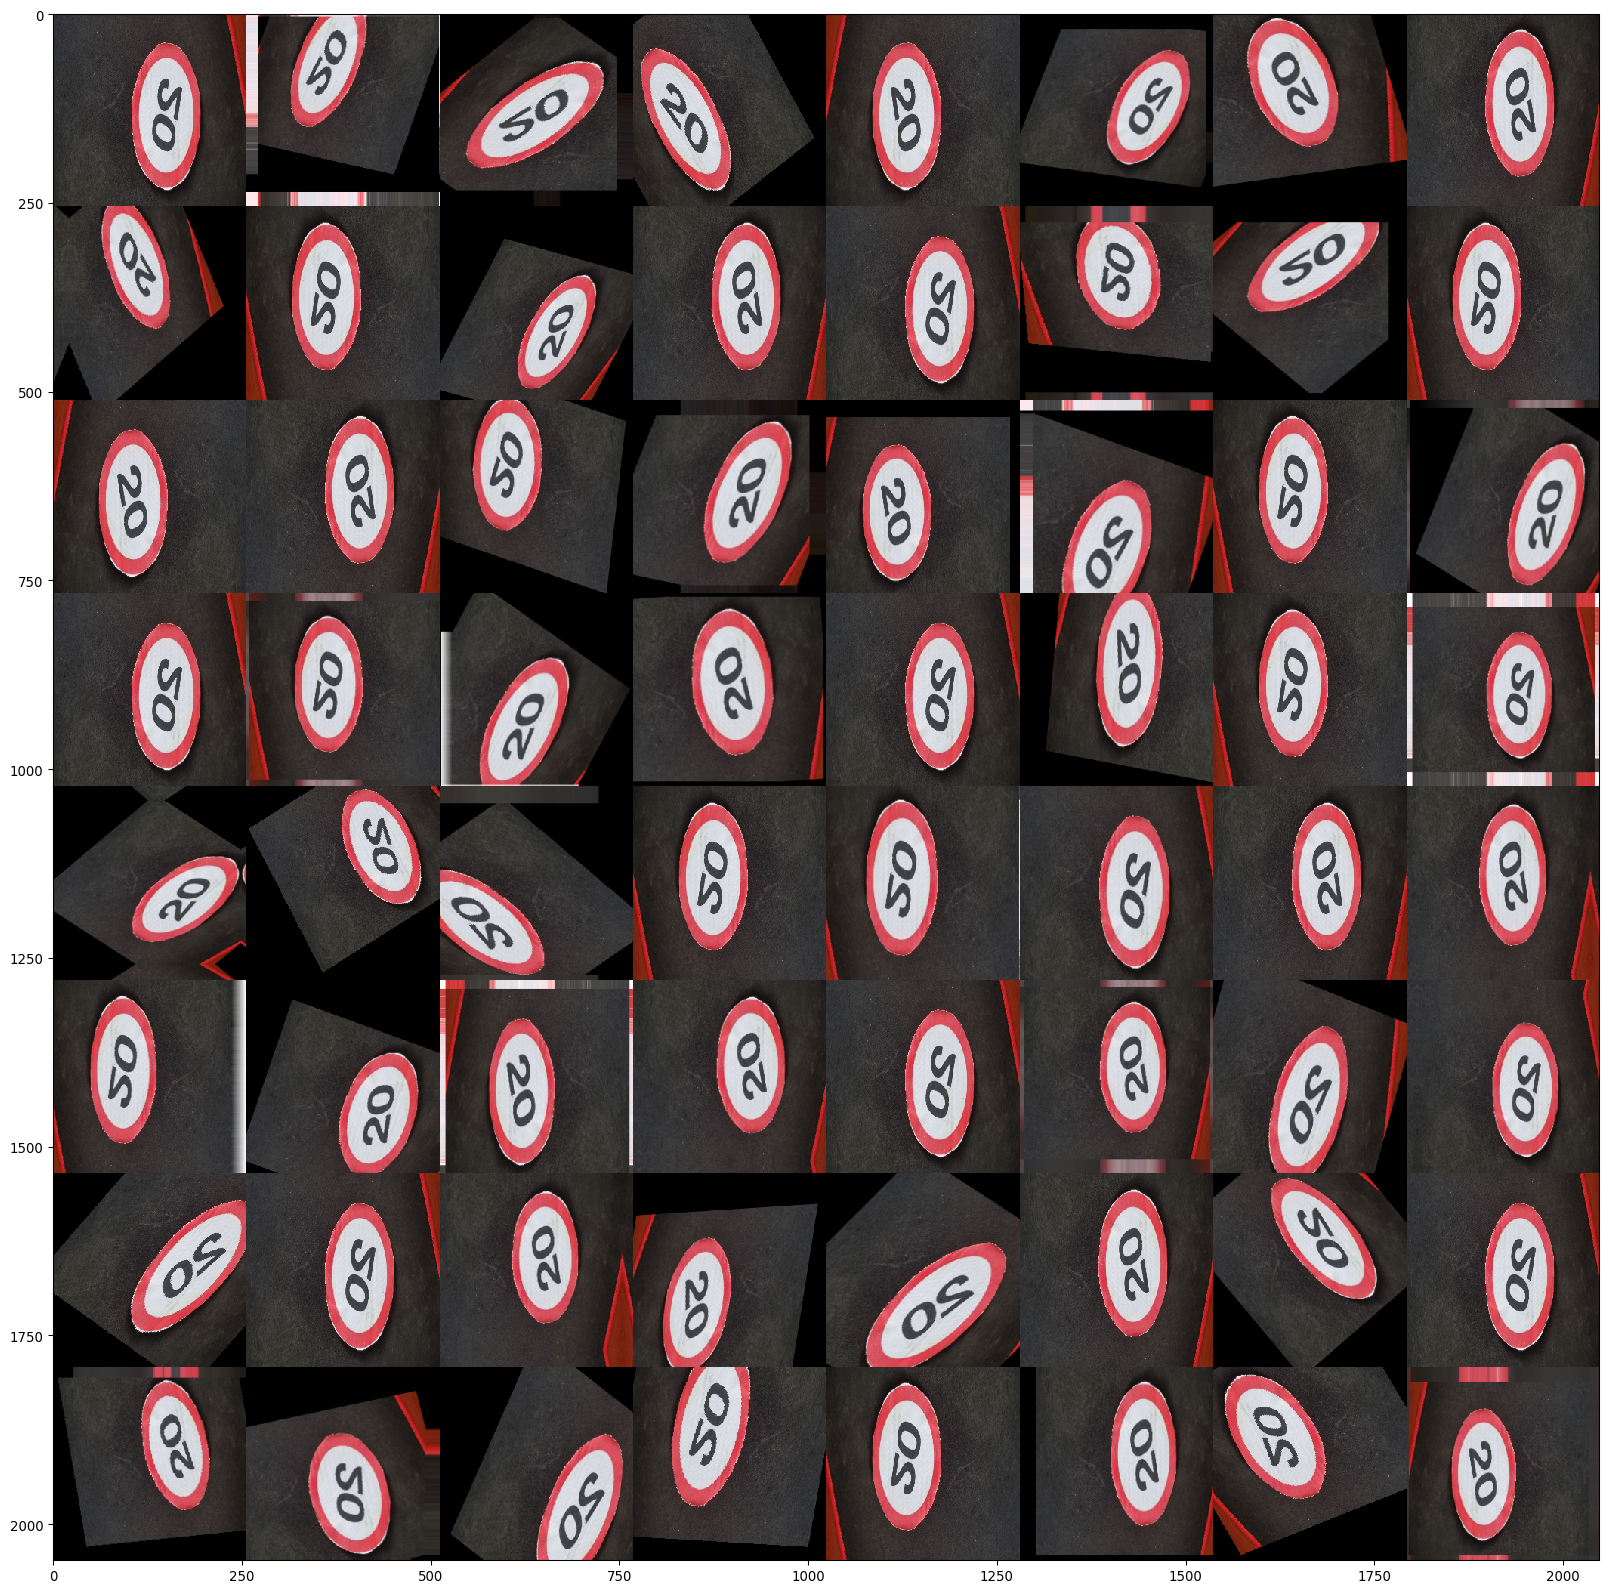
\includegraphics[width=\linewidth]{exdataaug}
      \caption{Example of the aurgemented img}
      \label{fig:augimg}

\end{figure}

\section{Results}

given the Table~\ref{Tab:result} we could observe the model AlexNet with the AdaDelta optimizer and the learning rate decay exponencial with the 0.99 rate
has a better Accuracy$\times$Performace. This one was used to classify the Traffic Signs Data set.\\
The result in the training (Fig:\ref{fig:alexnettraining}, Fig:\ref{fig:traffictraining})was very similar with the provided dataset. A bigger testset is need to provided a better
accuracy but all 3 pictures separated to the test have ben right classified.



\section{Conclusion}

We could see with almost every optimizer the GoogLeNet take more time to training the 10 epochs but it is meet a sable
curve a little before. Another point we can put out is the inference time almost in every case the GoogLeNet take more
time to infer and this not bring more accuracy to the model.
This maybe is related with the size of boths models, GoogLeNet is bigger and more complex Network.

\section{Future work}
\begin{itemize}
  \item Use the GTSRB dataset instead, this one was many mores classes.  
  \item Detection of the traffic signs and Classification.
  \item Use the different models, who wad a better performace in the traffic sign classsification.
  \item Try to deploy the detection and classification in a car in real time.
\end{itemize}


\begin{figure}[thpb]
      \centering
      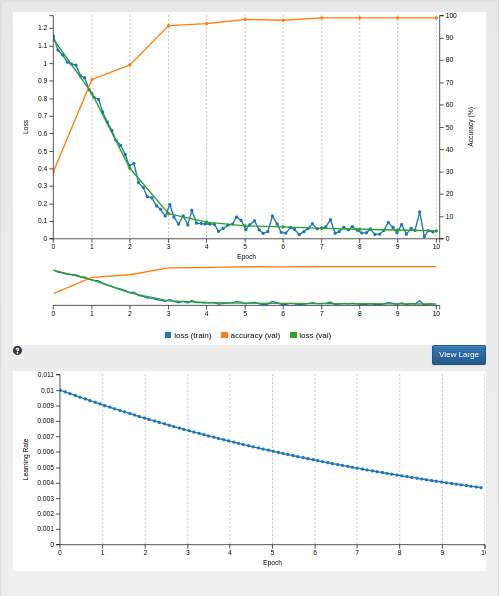
\includegraphics[width=\linewidth]{alex-10-adadelta-exp99-training.jpg}
      \caption{AlexNet-AdaDelta Training}
      \label{fig:alexnettraining}

\end{figure}

\begin{figure}[thpb]
      \centering
      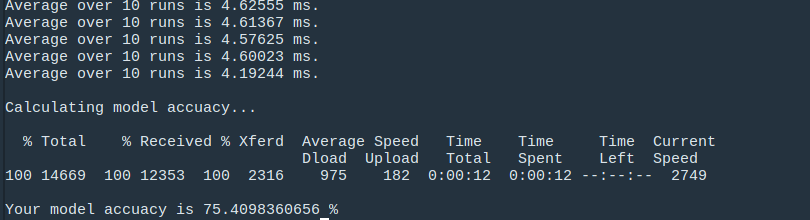
\includegraphics[width=\linewidth]{alex-10-adadelta-exp99-evaluate.jpg}
      \caption{AlexNet-AdaDelta Evalauate}
      \label{fig:alexnetevaluate}

\end{figure}

\begin{figure}[thpb]
      \centering
      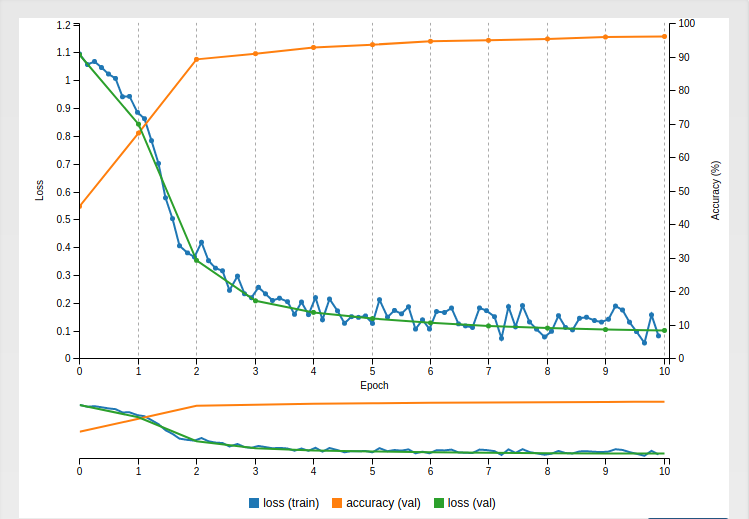
\includegraphics[width=\linewidth]{TrafficSigns-AlexNet-10-AdaDelta-Exp99-Training.jpg}
      \caption{Traffic Signs AlexNet-AdaDelta Training}
      \label{fig:traffictraining}

\end{figure}
%example for building table
    \begin{table}[ht]
\caption{Models comparative}
\begin{center}
\begin{tabular}{|c||c c c c c c|}
\hline
  Model & Optmizer & Decay & Time (10 Epoch) & Epoch steady & Inference Time & Accuracy\\

\hline
  \multirow{4}{4em}{Goog LeNet} 
  & SGD & Step 33 & 18 & 3 & 7.75 & 73.77 \\ 
  & Adam & Step 33 & 6 & 2 & 4.1 & 65.23 \\
  & AdaGrad & Step 33 & 18 & 3 & 9.55 & 75.41\\
  & AdaDelta & Exp .99 & 19 & 6 & 5.33 & 75.41\\
\hline
  \multirow{4}{4em}{AlexNet}
  & SGD & Step 33 & 6 & 4 & 8.55 & 73.77 \\ 

  & Adam & Step 33 & 6 & 1 & 3.43 & 67.21 \\
  & AdaGrad & Step 33 & 6 & 4 & 5.35 & 75.41\\
  & AdaDelta & Exp .99 & 6 & 7 & 4.57 & 75.40\\
\hline
\end{tabular}
\label{Tab:result}
\end{center}
\end{table}

\bibliography{bib}
\bibliographystyle{ieeetr}


\end{document}
